<<echo=FALSE, cache=FALSE>>=
set_parent('./project.Rnw')
@
%
To measure the performance and explore how well theory and practice coincide, the methods discussed was trained and tested on the Spam dataset \citep{Spamdata}. 

Most computations were run on a sever, and as a result the computation times were too inaccurate to be presented as results. They were therefore omitted from the report.
\\
\\
The most important part of the code used in the experiments can be found in Appendix~\ref{chap:Code}. It is primarily included so the reader can check which parameters were used. The full code can be found at github\footnote{\url{https://github.com/havakv/Project/tree/master/code/spam}}.


\section{Spam dataset}
\label{sec:Spam dataset}
 The Spam dataset is qute common in the machine learning world. 
 Each data point corresponds to an email, with a binary response telling if an email is spam or not. There are a total of 4601 data points and 57 predictors:
 \begin{itemize}
   \item 48 continuous real $[0, 100]$ corresponding to words. Each giving the percentage of words in the email matching that word. 
   \item 6 continuous real $[0, 100]$ corresponding to characters. Each giving the percentage of characters in the email matching that character.
   \item 1 continuous real $[1, \ldots]$ giving average length of uninterrupted sequences of capital letters. 
   \item 1 continuous integer $[1, \ldots]$ giving length of longest uninterrupted sequence of capital letters.
   \item 1 continuous integer $[1, \ldots]$ giving total number of capital letters in the email.
 \end{itemize}
 For more information on the dataset see \cite{Spamdata}.

 In the tests that follow, the Spam data was split into a training and test set of equal size. The algorithms were first trained on the training set, and then test error was plotted in form of $0/1$ misclassification error rate, i.e.
 \begin{align}
   \label{eq:missClassErr} 
   error =  \frac{1}{n_{test}} \sum_{i = 1}^{n_{test}} I\{C(\mathbf{x}_i) \neq y_i\}.
 \end{align}
 Here $C(\mathbf{x}_i)$ is the prediction based on $\mathbf{x}_i$, and $n_{test}$ is the number of test points. 
All methods were trained using the same data points. 
If the goal had been to actually make a spam filter, the error measure would not weight misclassification of spam and non-spam the same. Different costs for misclassification has not been the focus of this project, and for the purpose of testing the behavior of different methods \eqref{eq:missClassErr} is perfectly fine.


\section{CART}
\label{sec:CARTsim}
First classification trees were fitted to the data using \verb+rpart+ by \cite{rpart}. Large trees were grown using both the Gini index and deviance. They were then pruned back to a single node and the test errors for the different trees were plotted as function of the tree size in Figure~\ref{fig:cartCPSpam}. 
Both methods show how small trees are underfitted while large trees are overfitted, and somewhere in the middle, the optimal tree can be found. 
%
\begin{figure}[h!tp]
\begin{center}
    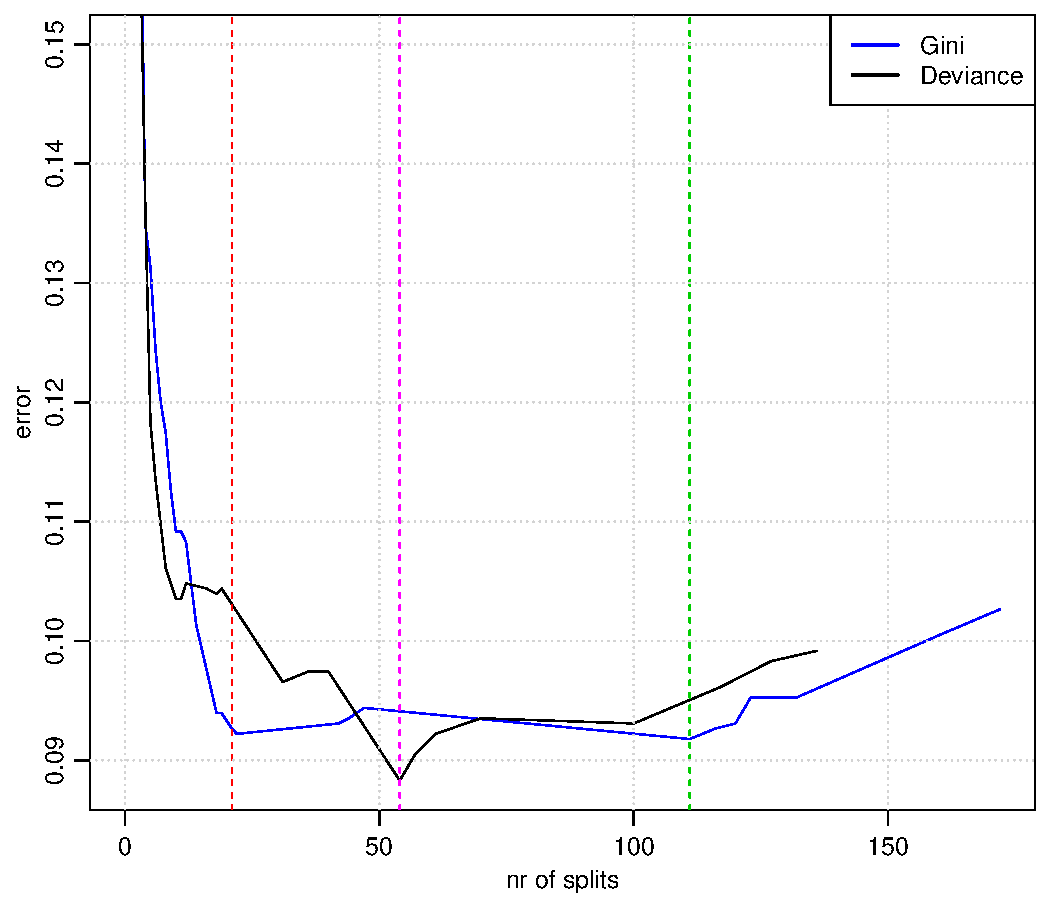
\includegraphics[scale=0.5]{./figures/cartCPSpam.pdf}
\end{center}
\caption{CART on Spam data. Test error as function of number of splits. The two lines represent trees grown with Gini index and deviance splitting criterion. A large tree is grown and the different points are test error of pruned trees depending on the tuning parameter $\alpha$ in \eqref{eq:CostPruning}. The green and magenta line marks the minima for the two lines. }
\label{fig:cartCPSpam}
\end{figure}
%

The green line marks the minimum test error using the Gini index. This graph is very flat around the minimum, so in terms of interpretability, a smaller tree can be chosen without sacrificing much of the predicting power. In Figure~\ref{fig:CartSpam}, the optimal tree (green) is displayed along with the tree from the red line (red). Their performance is almost identical, but the red tree give a nicer view of the data. Usually the trees are plotted with the splits like in Figure~\ref{fig:cart}. Here, they are left out because they serve no purpose in the context of the experiment. If the goal was to find which factors were most important in terms of classifying spam, they would be investigated more closely.

The magenta tree in Figure~\ref{fig:CartSpam}, is the tree grown using deviance in Figure~\ref{fig:cartCPSpam} corresponding to the magenta line. In this experiment, it outperforms all the Gini trees, though only barely. 

\begin{figure}[htb]
  \centering
  \begin{subfigure}[b]{0.48\textwidth}
    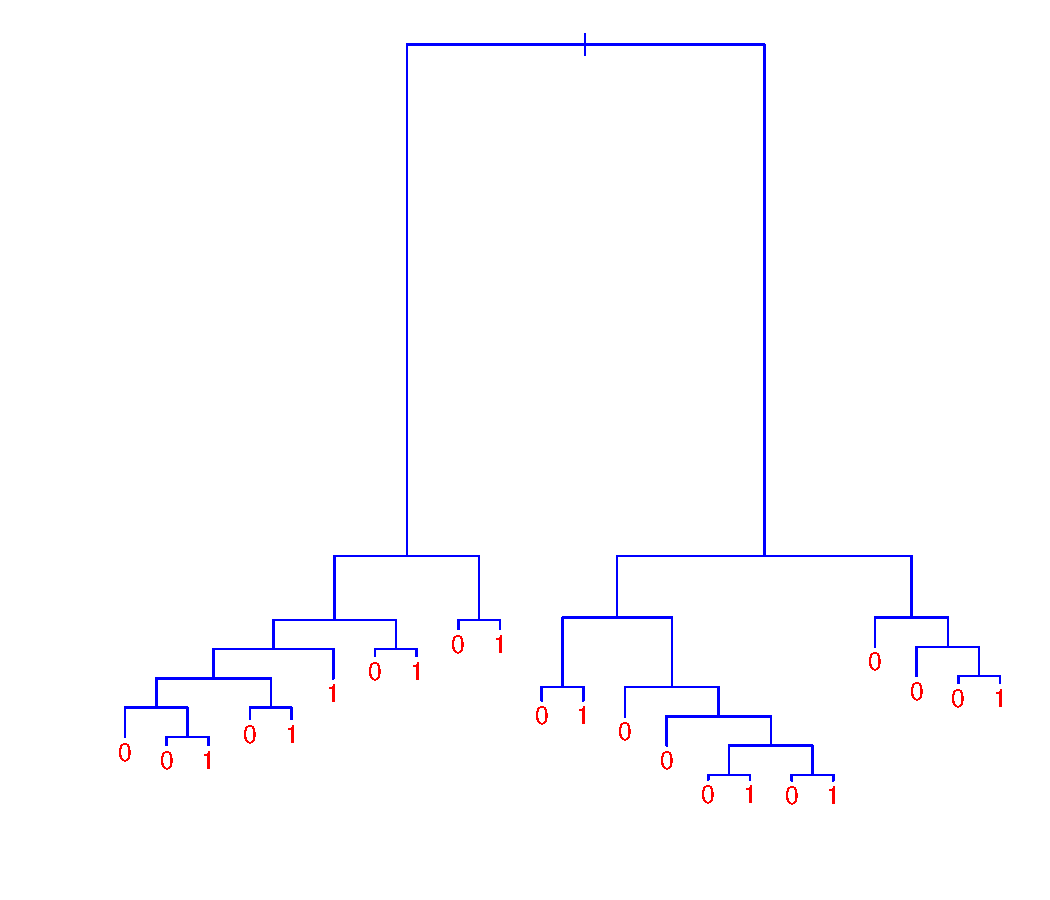
\includegraphics[width=\textwidth]{./figures/cartSmallSpam.pdf}
  \end{subfigure}%
  \quad
  \begin{subfigure}[b]{0.48\textwidth}
    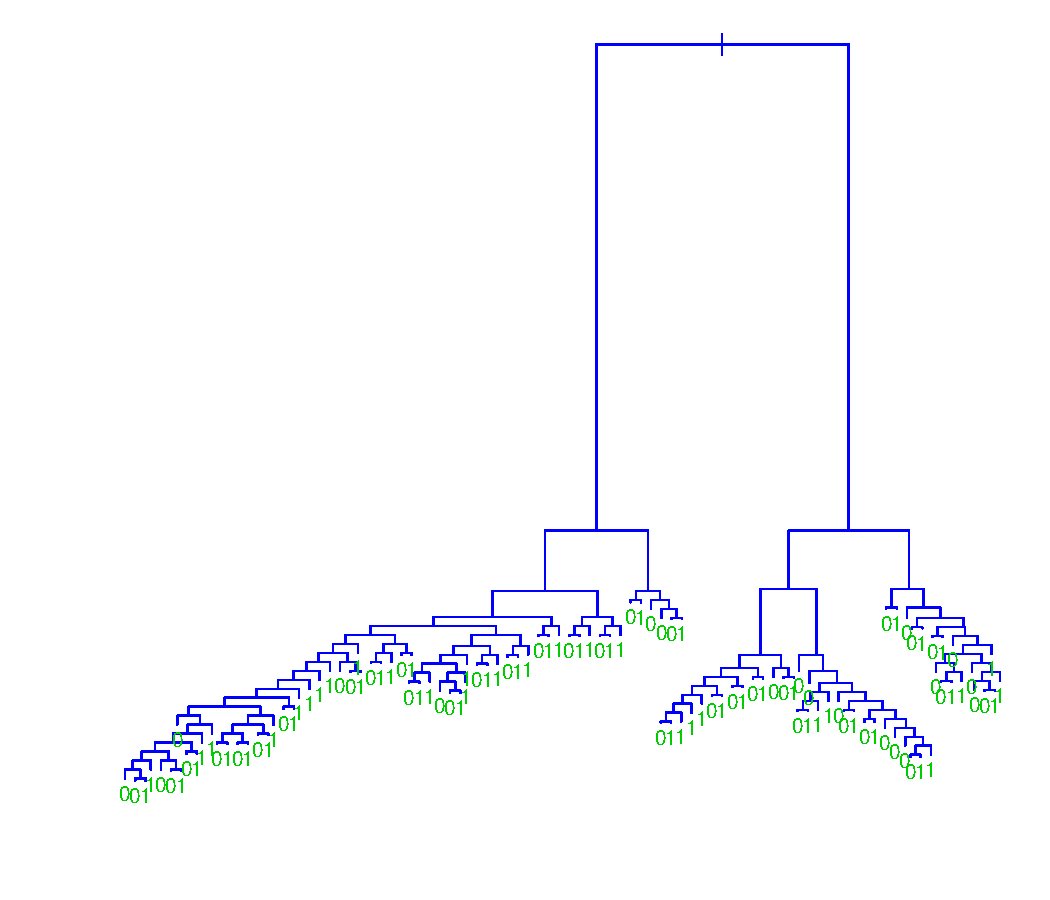
\includegraphics[width=\textwidth]{./figures/cartOptSpam.pdf}
  \end{subfigure}
  \quad
  \begin{subfigure}[b]{0.48\textwidth}
    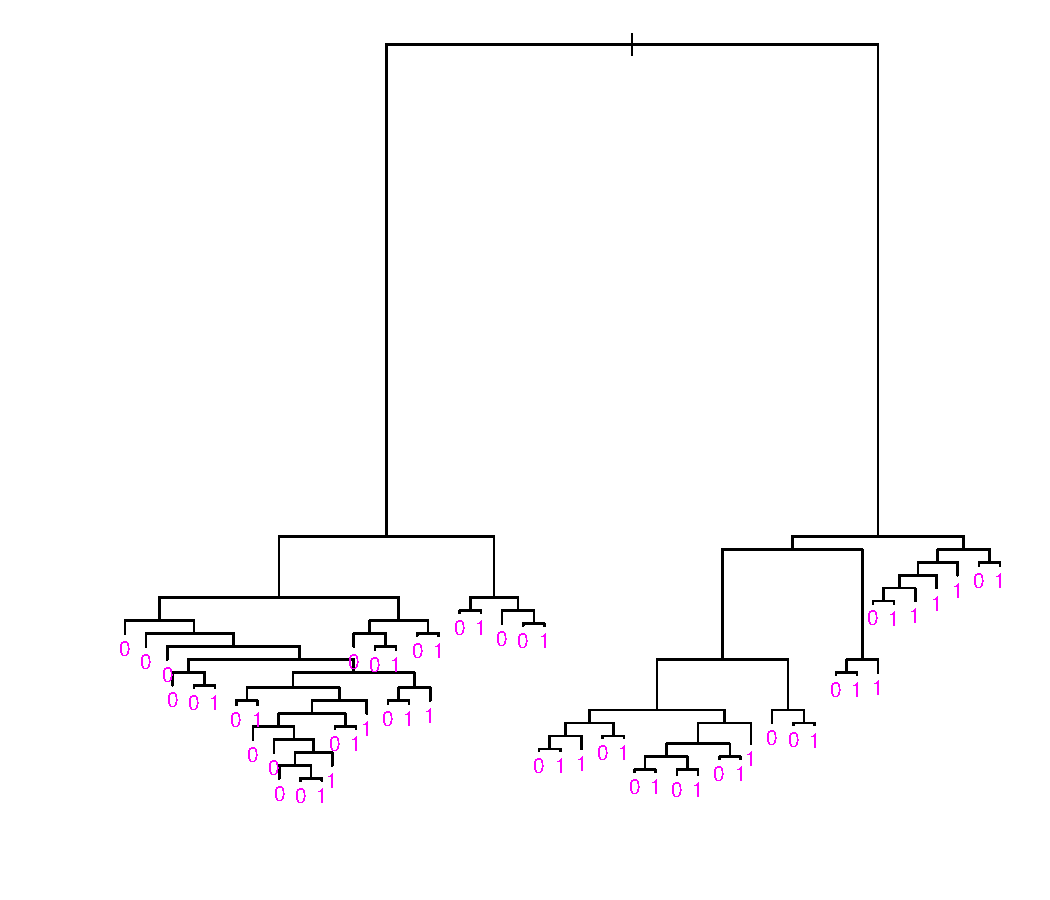
\includegraphics[width=\textwidth]{./figures/cartOptDevianceSpam.pdf}
  \end{subfigure}
          %(or a blank line to force the subfigure onto a new line)
  \vspace{1\baselineskip}
  \caption{CART on Spam data. Trees from \ref{fig:cartCPSpam} are displayed. The green tree has the minimal test error using the Ginie index, while the red have a much simpler structure with almost the same test error. The magenta tree is the best performing using the deviance splitting criterion.}
  \label{fig:CartSpam}
\end{figure}


\section{Adaboost}
\label{sec:SimAdaBoost}
Adaboost was fitted to the Spam data using the \verb+boosting+ function in \verb+adabag+ by \cite{adabag}. It use the \verb+rpart+ implementation of CART as base classifiers. The main tuning parameters in Adaboost are the number of iterations, and the tree depth. In Figure~\ref{fig:adaboostSpam}, the test error is plotted as function of iterations, for different tree depths. It is clear that the algorithm does pretty well after few iterations, and outperforms CART easily. Only a maximum of 300 iterations were done, but by the look of it, Adaboost seems quite robust to overfitting. 

Surprisingly, Adaboost does better for deeper trees. It is expected to overfit for larger trees, but it does not. One possible explanation could be that there are higher order interactions between the features in the dataset (see Section~\ref{sub:Tree size}). 

In this case, depth refers to them maximum number of successive splits. So the root node as depth 0, its children depth 1 and so on.
It is not possible to fit trees deeper than $30$ in the \verb+boosting+ function, but it would have been interesting to see how the performance developed for even deeper trees. 
%
\begin{figure}[htbp]
\begin{center}
    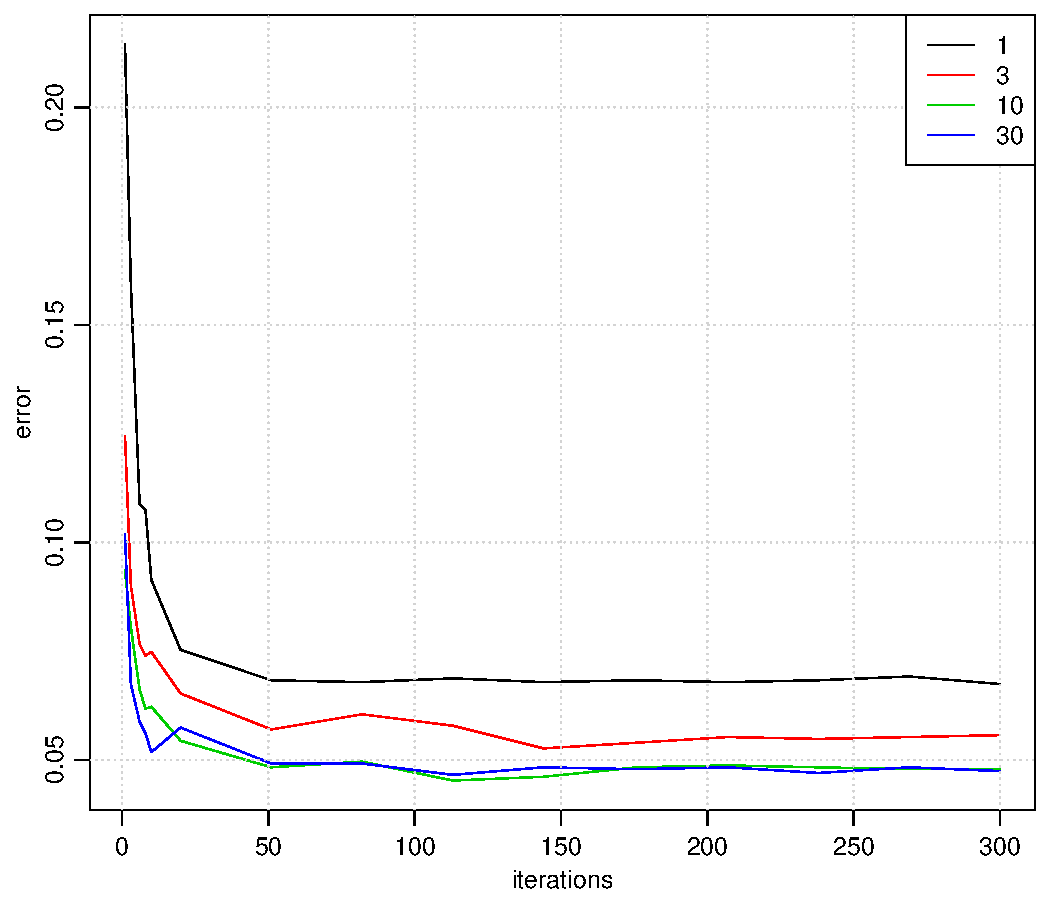
\includegraphics[scale=0.5]{./figures/adaboostSpam.pdf}
\end{center}
\caption{Adaboost on Spam data. Each line represent a tree depth.}
\label{fig:adaboostSpam}
\end{figure}
%
\section{Gradient Boosting}
\label{sec:SimGradBoost}
Gradient Boosting is a very powerful method, but requires some tuning. The goal here was not to find the optimal tuning parameters for the Spam dataset, but rather to investigate the effect of changing different parameters. The package \verb+gbm+ by \cite{gbm} was used to fit the Gradient Boosting with deviance loss.

\begin{figure}[htbp]
  \centering
  \begin{subfigure}[b]{0.48\textwidth}
    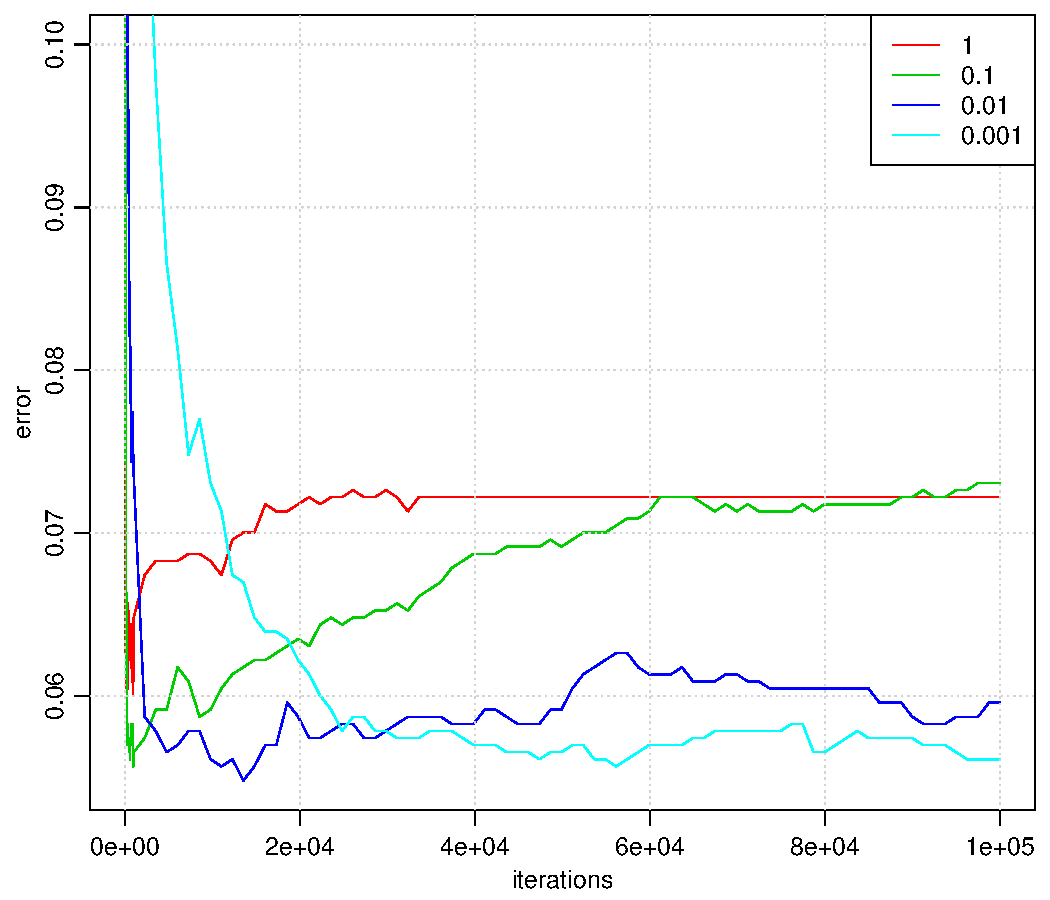
\includegraphics[width=\textwidth]{./figures/gradboostSpamShrink2.pdf}
    \caption{Different shrinkages $\nu$.}
    \label{fig:gradboostSpamShrink2}
  \end{subfigure}%
  \quad
  \begin{subfigure}[b]{0.48\textwidth}
    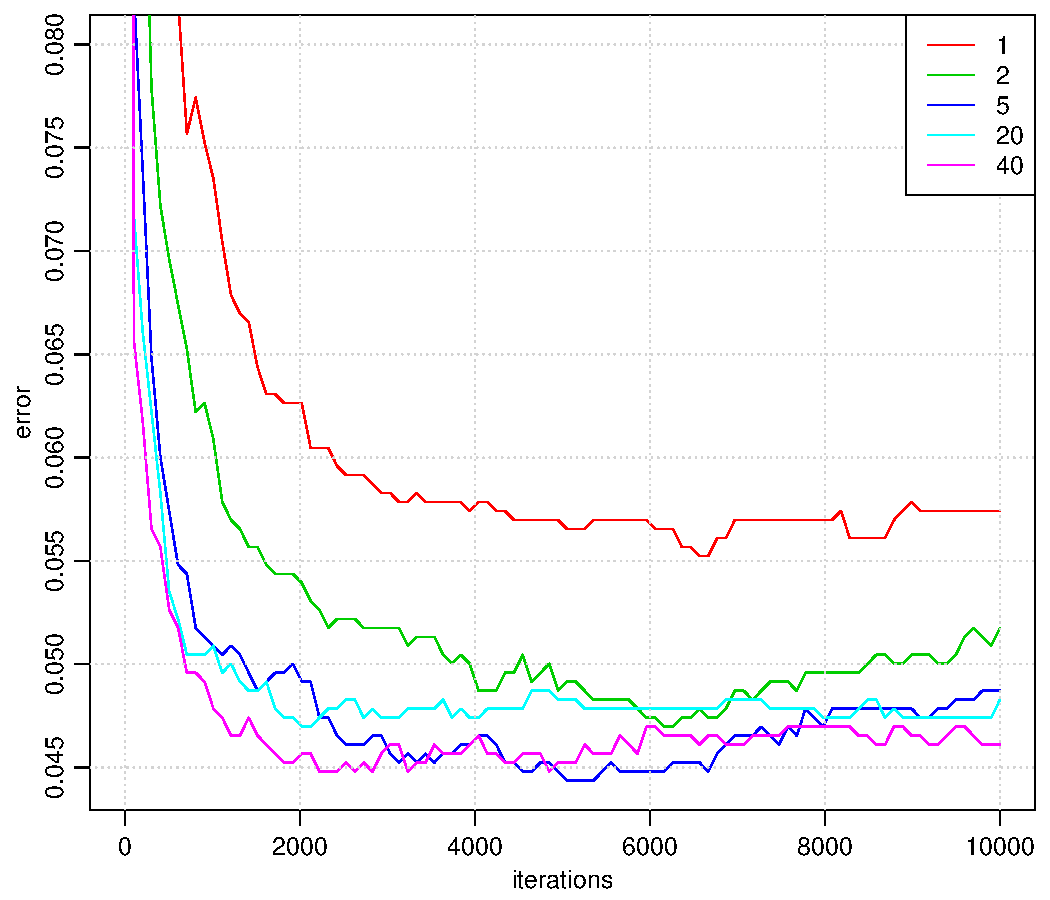
\includegraphics[width=\textwidth]{./figures/gradboostSpamDepth.pdf}
    \caption{Different tree depths.}
    \label{fig:gradboostSpamDepth}
  \end{subfigure}
          %(or a blank line to force the subfigure onto a new line)
  \vspace{1\baselineskip}
  \caption{Gradient Boosting on Spam data.}
  \label{fig:GradBoostSpam}
\end{figure}

The optimal number of iterations is highly dependent on the shrinkage parameter (see Section~\ref{sub:Shrinkage}). In Figure~\ref{fig:gradboostSpamShrink2} the test error is plotted against number of boosting iterations. Each line represent a different shrinkage. It is clear from the plot that for lower shrinkage, more iterations are needed. This means shrinkage is costly in terms of computations. However, the worst performing line is that without shrinkage ($\nu = 1$), though the difference is quite small. The figure indicates that, for the Spam data, there is no point with $\nu < 0.1$, as there is no gain in test error.

Studying the lines with shrinkage 1 and 0.1, it is clear that Gradient Boosting can overfitt. However, many iterations are needed, so there is no evidence here that it is more prone to overfitting than Adaboost.
\\
\\
As with Adaboost, the tree depths are important to to consider. In Figure~\ref{fig:gradboostSpamDepth} test error for different tree depths are displayed. \verb+gbm+ does not take depth as a parameter, but instead the parameter \verb+interaction.depth+. It represents the interactions discussed in Section~\ref{sub:Tree size}, where $1$ is an additive model, $2$ is a model with up to second order interactions, and so on. In principle \verb+interaction.depth+$+1$ gives the maximum number of terminal nodes.

The figure shows the same trend as Adaboost did. Deeper trees give better results, though the difference is much smaller than for Adaboost.
\\
%
\begin{figure}[htbp]
\begin{center}
    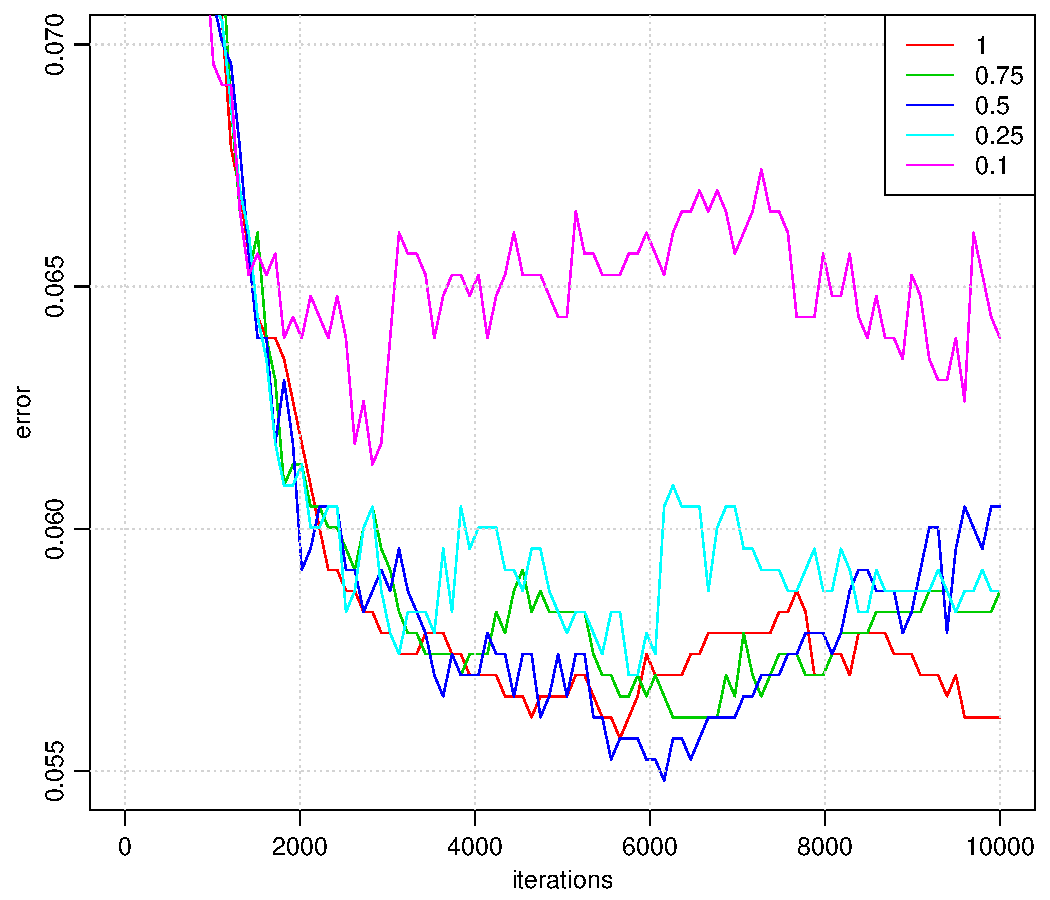
\includegraphics[scale=0.5]{./figures/gradboostSpamStoch.pdf}
\end{center}
\caption{Stochastic Gradient Boosting on Spam data. The sample fractions are specified in the legend.}
\label{fig:StochasticGradBoost}
\end{figure}
\\
Stochastic Gradient Boosting was mentioned as a minor modification of Gradient Boosting in Section~\ref{sec:Stochastic Gradient Boosting}. The only difference is that a subset of the training data is drawn at each iteration. \verb+gbm+ refers to this parameter as the \verb+bag.fraction+. In Figure~\ref{fig:StochasticGradBoost}, the test error is plotted for different sample sizes, where \verb+bag.fraction+ gives the fraction of the dataset sampled. The figure does not show any improvement in test error from introducing randomness. However, for subset fractions down to $0.5$ the performance does not drop. As the number of computations decreases with smaller fractions, there is still some gain in doing Stochastic Gradient Boosting here.

\section{Bagging and Random Forests}
\label{sec:BaggandRFSim}
Random Forests is more or less an extension of Bagging, and tries to improve performance through decorrelating the trees. In Figure~\ref{fig:baggingAndRFSpam} both methods were fitted to the Spam data using \verb+ipred+ by \cite{ipred} and \verb+randomForest+ by \cite{randomForestR}. The default tuning parameters were used for the methods. The figure shows how the test error changes with number of trees used. Here Random Forest slightly outperform Bagging, which is as expected, and both are a vast improvement of CART. There is no sign that either method is overfitting as the number of trees increase, which coincide with the theory in Section~\ref{sub:Overfitting}.
\\
\begin{figure}[htbp]
  \centering
  \begin{subfigure}[b]{0.48\textwidth}
    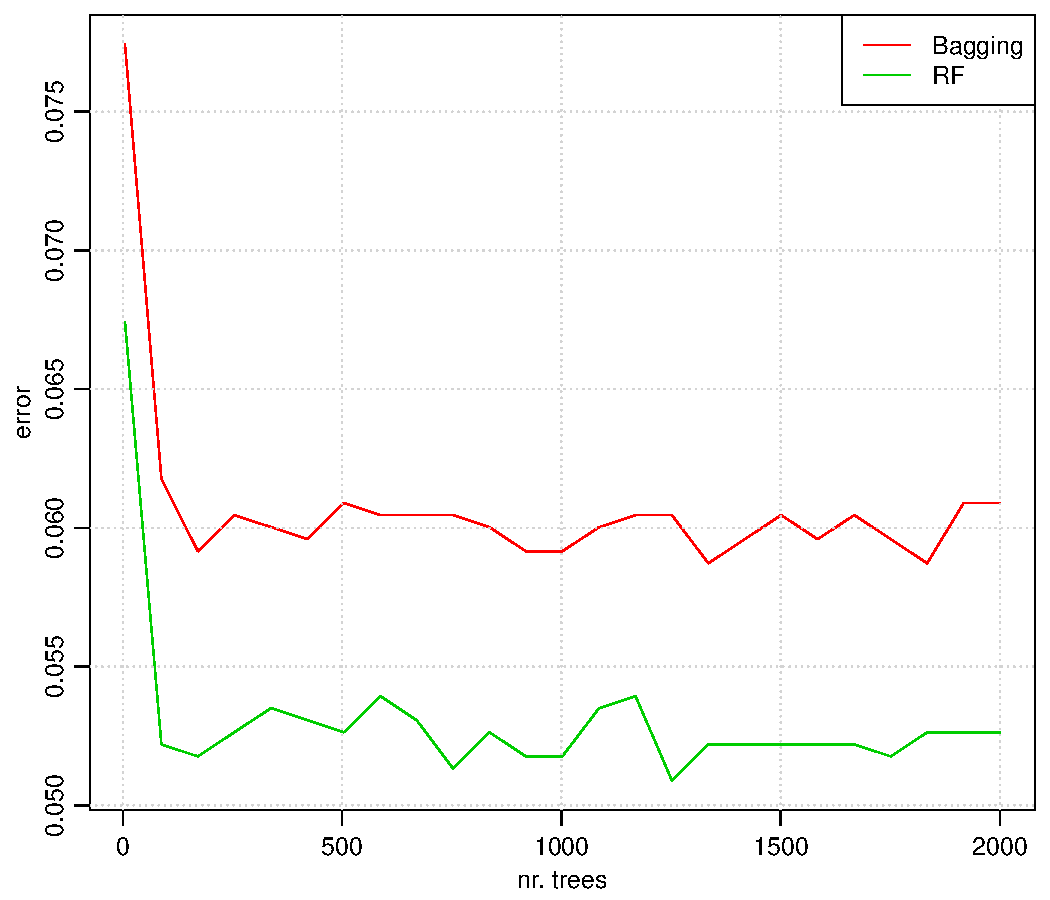
\includegraphics[width=\textwidth]{./figures/baggingAndRFSpam.pdf}
    \caption{Test error as function of bootstrap samples for Bagging and RF.}
    \label{fig:baggingAndRFSpam}
  \end{subfigure}%
  \quad
  \begin{subfigure}[b]{0.48\textwidth}
    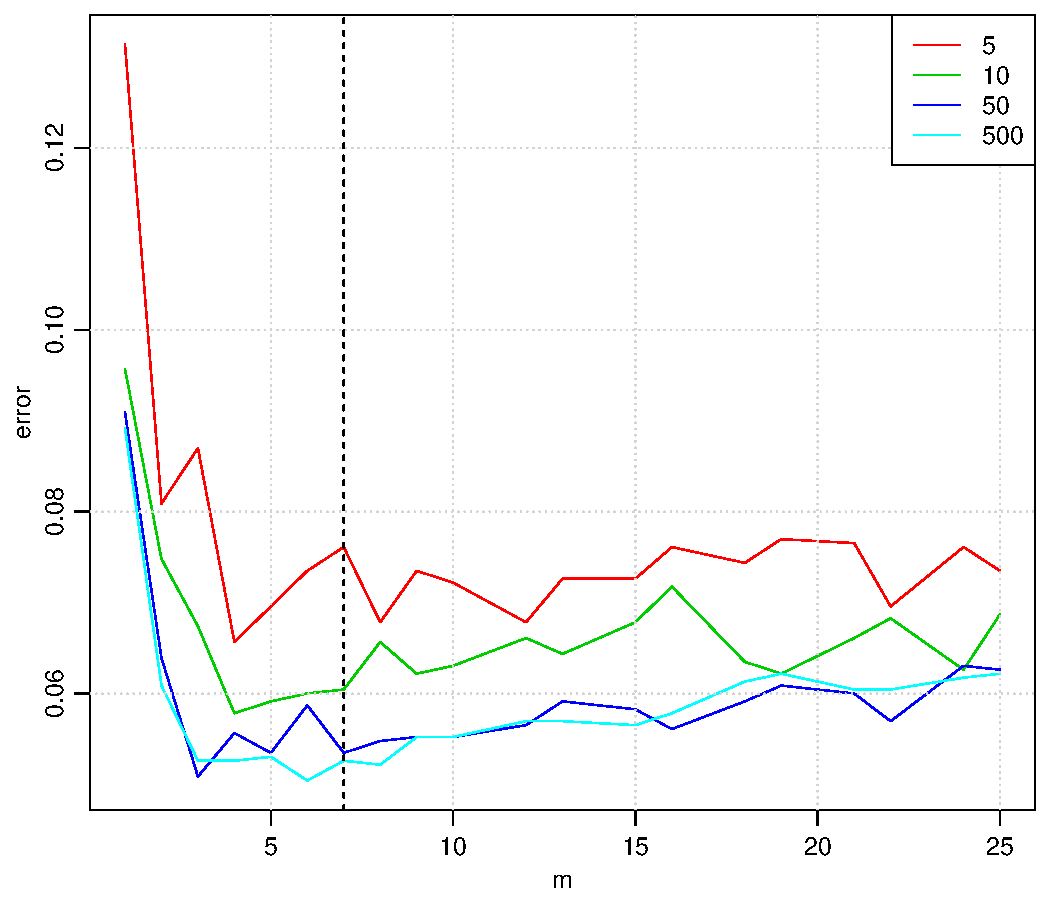
\includegraphics[width=\textwidth]{./figures/RFSpam.pdf}
    \caption{RF as func. of m, for different number of bootstrap samples. Vertical line marks $\lfloor \sqrt{p} \rfloor$.}
    \label{fig:RFSpam}
  \end{subfigure}
          %(or a blank line to force the subfigure onto a new line)
  \vspace{1\baselineskip}
  \caption{Bagging and Random Forests on Spam data.}
  \label{fig:baggAndRF}
\end{figure}
\\
Figure~\ref{fig:RFSpam} shows how the number of randomly chosen features $m$ affects the test error. This is done for different number of trees, and the vertical line marks the default value $m = \lfloor \sqrt{p} \rfloor$. In this case the default value for $m$ is maybe a bit high, but it is more or less equal to the optimal value and defends its position as a default parameter value well. 
\\
\begin{figure}[htpb]
\begin{center}
    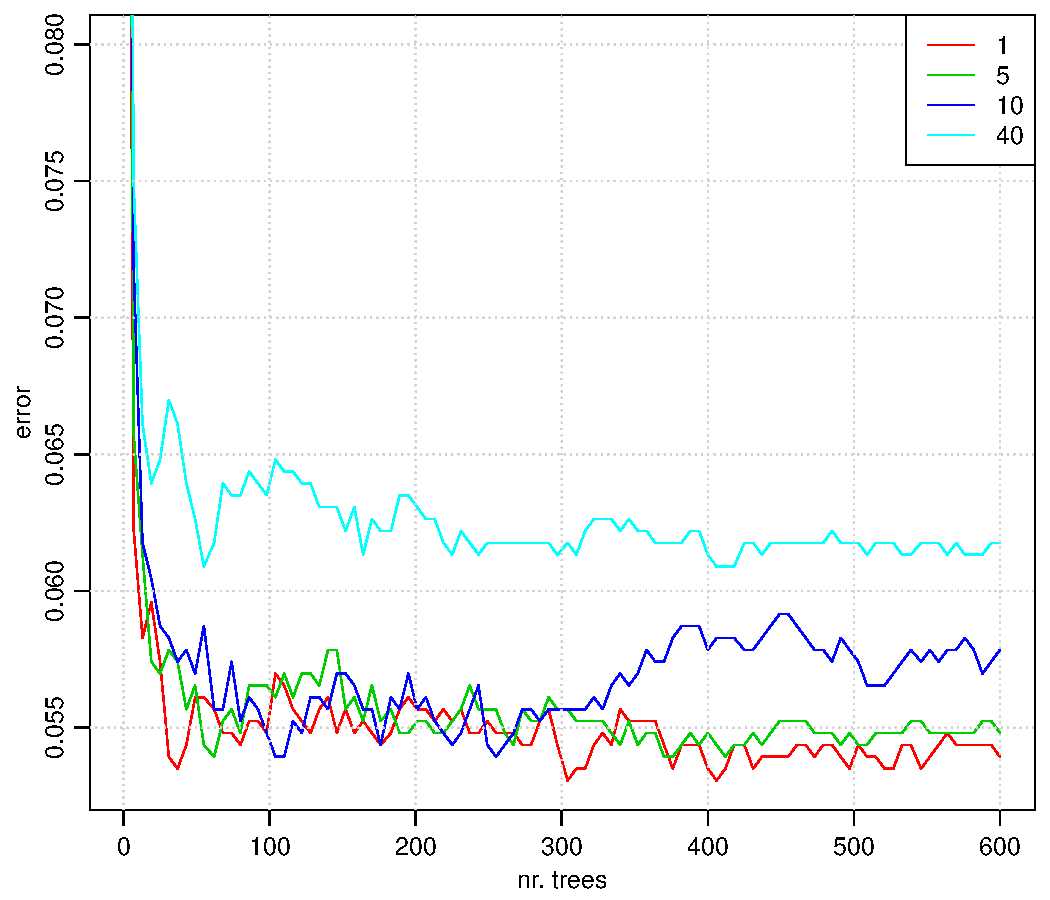
\includegraphics[scale=0.5]{./figures/RFTreeDepth.pdf}
\end{center}
\caption{Random Forests on Spam data, with different tree depths. The numbers in the legend indicates the minimum number of nodes in a terminal node.}
\label{fig:RFTreeDepth}
\end{figure}
\\
As discussed in Section~\ref{sub:Overfitting}, Bagging and Random Forests can be overfitted in terms of overfitting the individual trees. Figure~\ref{fig:RFTreeDepth} show the test error for 4 different tree depths. The \verb+randomForest+ package does not take depth as an argument, but instead the minimum number of training points in each terminal node. So the red line corresponds to a fully grown tree. The figure shows that there is no gain in restricting the size of the trees for the Spam data. For high restrictions (see light blue line 40), unnecessary bias is introduced and the performance drops.  As Bagging and Random Forests are so similar, the experiment was not repeated with bagging.
\\
\\
In Section~\ref{sub:Out-of-bag}, the Out-of-bag error was introduced as an approximation of the test error. It has very little computational cost and can replace cross-validation in tuning of parameters. Figure~\ref{fig:OOBvsTestvsCV} shows OOB, test error, and 10-fold cross-validation error for Random Forest on the Spam data. 
OOB error is also available for Stochastic Gradient Boosting and Bagging, but only Random Forests was tested here.
The figure shows that both OOB and 10-fold cross-validated error are good approximations for the test error. This means that OOB can be used as a check of when the test error has converged and no more trees are needed. 

\begin{figure}[htbp]
\begin{center}
    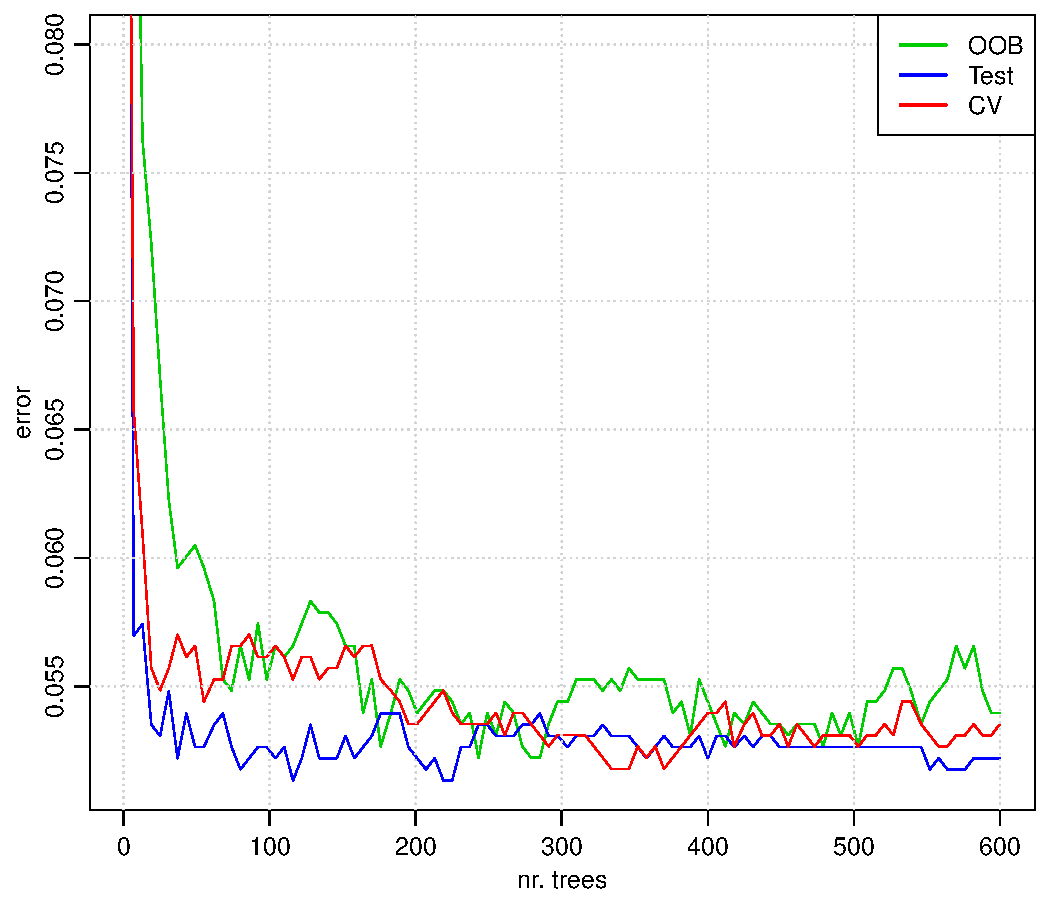
\includegraphics[scale=0.5]{./figures/OOBvsTestvsCV.pdf}
\end{center}
\caption{Out-of-bag, 10-fold cross-validation and test error for Random Forests on Spam data.}
\label{fig:OOBvsTestvsCV}
\end{figure}

Figure~\ref{fig:OOBvsTestvsCV} only shows \textit{one} run. As there is a lot of randomness in the methods the lines varies somewhat between runs. Maybe a figure with bootstrapped confidence bounds would be a better choice in this context. This was not done as the figure perfectly illustrate its purpose as is. 

\section{Phoneme}
\label{sec:Phoneme}
All the experiments were repeated on the Phoneme dataset from \cite{phoneme}. 
The aim of this dataset is to distinguish between nasal (class 0) and oral sounds (class 1). The class distribution is 3,818 samples in class 0 and 1,586 samples in class 1. 

However, all the results coincide with the results from the Spam data. As a consequence, they do not contribute in any way to the report and are therefore not displayed. 


\clearpage

